\section{Implementation}\label{sec:implementation}

\subsection{Implementation Strategy}

\lang\ transpiles to OCaml and its implementation follows the structure of a
typical domain-specific language (DSL) compiler. Although \lang's current
implementation is not as an embedded DSL, its the general design is simple enough
to adapt to being so and also to target other languages.

Alongside the transpiler, a `Read-Check-Translate' loop, benchmarking program
and a test suite are included in the artifacts accompanying this paper.

\begin{enumerate}

    \item \textbf{Parsing}. A generated, LR(1) parser parses a text file into a
        syntax tree. In general, this part will vary for different languages
        and can also be dealt with using combinators or syntax-extensions (the
        EDSL approach) if the host language offers such support.

    \item \textbf{Desugaring}. The syntax tree is then desugared into a
        smaller, more concise, abstract syntax tree. This allows for the type
        checker to be simpler to specify and easier to implement.

    \item \textbf{Matrix Expressions} are also desugared into the abstract
        syntax tree through pattern-matching.

    \item \textbf{Type checking}. The abstract syntax tree is explicitly typed,
        with some inference to make writing typical programs more convenient.

    \item \textbf{Code Generation}. The abstract syntax tree is translated into
        OCaml, with a few `optimisations' to produce more readable code. This
        process is type-preserving: \lang's type system is embedded into
        OCaml's (Figure~\ref{fig:type_grammar}), so the OCaml type checker
        acts as a sanity check on the generated code.

\end{enumerate}

A very pleasant way to use \lang\ is to have the build system generate code at
\emph{compile-time} and then have the generated code be used by other modules
like normal OCaml functions. This makes it possible and even easy to use \lang\
alongside existing OCaml libraries; in fact, this is exactly how the
benchmarking program and test-suite use code written in \lang.

\subsubsection{Desugaring, Matrix Expressions and Type Checking}

As seen earlier (Figure~\ref{fig:lang_desugar}), desugaring is conventional.
Matrix expressions are translated into BLAS/LAPACK calls via purely syntactic
pattern-matching (also seen earlier in Figure~\ref{fig:lang_matexp}).

\subsubsection{Type checking}

Type checking is mostly standard for a linearly typed language,
with the exception of fractional permission inference. By restricting fractions
to be non-positive integer powers of two, we only need to keep track of the
logarithm of the fractions used. Explicit sharing and unsharing removes the
need for performing dataflow analysis. As a result, all fractional arithmetic
can be solved with unification, and in doing so, fractions become directly
usable in \lang's type-system as opposed to a convenient theoretical tool.

Because all functions must have their argument types explicitly annotated,
inferring the correct fraction at a call-site is simply a matter of
unification. We believe \emph{full-inference of fractional permissions is
similarly just matter of unification} (thanks to an experimental implementation
of just this feature), even though the formal system we present here is for an
explicitly-typed language.

There are a few differences between the type system as presented in
\ref{subsec:semantics} and how we implemented it: the environment
\emph{changes} as a result of type checking an expression (the standard
transformation to avoid a non-deterministic split of the environment for
checking pairs); variables are \emph{marked as used} rather than removed for
better error messages; variables are \emph{tagged} as linear or intuitionistic
in \emph{one} environment as opposed to being stored in \emph{two} separate
ones (this allows scoping/variable look-up to be handled uniformly).

\subsubsection{Code Generation}

Code generation is a straightforward mapping from \lang's core constructs to
high-level OCaml ones. We embed \lang's type- and term- constructors into OCaml
as a sanity check on the output (Figure~\ref{fig:type_grammar}).

\begin{figure}[t]
    \centering
    \begin{minipage}{.3\textwidth}
        \centering
        \begin{grammar}
            <f> ::= `'
            \alt <'fc>
            \alt `z'
            \alt <f> `s'

            <t> ::= `'
            \alt `unit'
            \alt `bool'
            \alt `int'
            \alt `elt'
            \alt <f> `arr'
            \alt <f> `mat'
            \alt `!' <t>
            \alt <'fc.> <t>
            \alt <t> \lit{$\otimes$} \synt{$t'$}
            \alt <t> \lit{$\multimap$} \synt{$t'$}
        \end{grammar}
    \end{minipage}
    \begin{minipage}{.3\textwidth}
        \centering
        \begin{minted}[fontsize=\small]{ocaml}
module Arr =
  Owl.Dense.Ndarray.D

type z = Z
type 'a s = Succ

type 'a arr =
  A of Arr.arr
  [@@unboxed]

type 'a mat =
  M of Arr.arr
  [@@unboxed]

type 'a bang =
  Many of 'a
  [@@unboxed]
        \end{minted}
    \end{minipage}
    \begin{minipage}{.3\textwidth}
        \begin{align*}
            [\![ '\!f\!c ]\!] &= \texttt{'fc} \\
            [\![ \textbf{z} ]\!] &= \texttt{z}\\
            [\![ f \, \textbf{s} ]\!] &= [\![ f ]\!]\, \texttt{s}\\
            [\![ \textbf{unit} ]\!] &= \texttt{unit}\\
            [\![ \textbf{bool} ]\!] &= \texttt{bool}\\
            [\![ \textbf{int} ]\!] &= \texttt{int}\\
            [\![ \textbf{elt} ]\!] &= \texttt{float}\\
            [\![ f\, \textbf{arr} ]\!] &= [\![ f ]\!]\, \texttt{arr}\\
            [\![ f\, \textbf{mat} ]\!] &= [\![ f ]\!]\, \texttt{mat}\\
            [\![ \textbf{!} \, t ]\!] &= [\![ t ]\!]\, \texttt{bang}\\
            [\![  '\!f\!c.\, t ]\!] &= [\![ t ]\!]\\
            [\![ t \otimes t' ]\!] &= [\![ t ]\!] \texttt{*} [\![ t' ]\!]\\
            [\![ t \multimap t' ]\!] &= [\![ t ]\!] \rightarrow [\![ t' ]\!]
        \end{align*}
    \end{minipage}
    \caption{\lang's type grammar (left) and its embedding into OCaml
        (right).}\label{fig:type_grammar}
\end{figure}

This is also useful when using \lang\ from within OCaml; for example, we can
use existing tools to inspect the type of the function we are using
(Figure~\ref{fig:build}). It is worth reiterating that only the type- and term-
constructors are translated into OCaml, \lang's precise control over linearity
and aliasing are not brought over.

\begin{figure}[t]
    \centering
    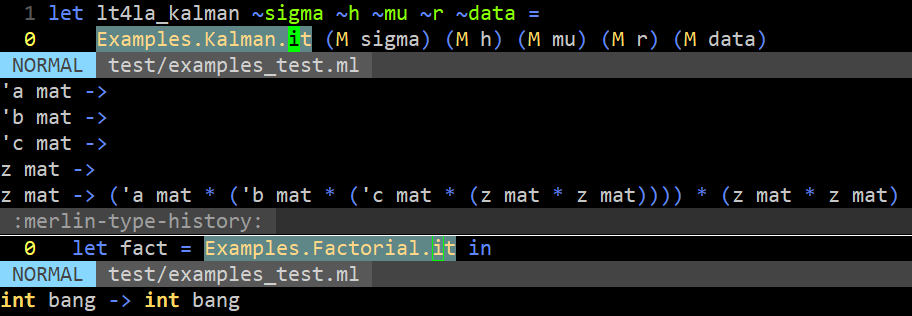
\includegraphics[width=\textwidth]{impl_build}
    \caption{Using \lang\ functions from OCaml.}\label{fig:build}
\end{figure}

We actually use this fact to our advantage to clean up the output OCaml by
removing what would otherwise be redundant re-bindings
(Figure~\ref{fig:lang_optimise}).  Combined with a code-formatter, the
resulting code is not obviously correct and exactly what an expert would intend
to write by hand, but now with the guarantees and safety of \lang\ behind it. A
small example is shown in Figure~\ref{fig:ocaml_sumarray}, a larger one in
Figure~\ref{fig:ocaml_kalman}.

\begin{figure}[t]
\begin{center}
    \begin{tabular}{rcl}
        \alsocell[b]{l}{\highl{let Many x = x in} \\
        \highl{let Many x = Many (Many x) in <exp>} } &
        $\Rightarrow$ &
        \highl{<exp>}
    \\ \\
        \alsocell[c]{l}{\highl{(* fixp = fix (f, x:t, <exp> : t') *)} \\
            \highl{(*1*) let Many f = Many fixp in <body>} \\
            \highl{(*2*) let f = fixp in <body>} } &
        $\Rightarrow$ &
        \highl{let rec f x = <exp> in <body>}
    \\ \\
    \alsocell[c]{l}{\highl{(*1*) let Many x = <exp> in} \\
            \highl{(*-*) let Many x = Many (Many x) in <body>} \\
            \highl{(*2*) let Many x = Many <exp> in <body>} \\
            \highl{(*3*) (fun x : t -> <body>) <exp>}} &
        $\Rightarrow$ &
        \highl{let x = <exp> in <body>}
    \end{tabular}
\end{center}
\caption{Removing redundant re-bindings during translation to OCaml.}\label{fig:lang_optimise}
\end{figure}

\begin{figure}[tp]
    \centering
    \begin{minted}[fontsize=\small]{ocaml}
let rec sum_array i n x0 row =
  if Prim.extract @@ Prim.eqI i n then (row, x0)
  else
    let row, x1 = Prim.get row i in
    sum_array (Prim.addI i (Many 1)) n (Prim.addE x0 x1) row in
sum_array
    \end{minted}
    \caption{Recursive OCaml function for a summing over an array, generated (at
        \emph{compile time}) from the code in Figure~\ref{fig:lang_sumarray},
        passed through \texttt{ocamlformat} for presentation.}\label{fig:ocaml_sumarray}
\end{figure}

\subsection{Performance Metrics}

We think that using \lang\ has two primary benefits: safety and performance. We
discuss safety in \ref{subsec:finding_bugs}, where we describe how we used
\lang\ to find linearity and aliasing bugs in a linear algebra algorithm that
was \emph{generated} by another program.

\subsubsection{Setup}

For performance, we measured the execution times of four equivalent
implementations of a Kalman filter: in C (using \textsc{Cblas}), \lang\ (using
\textsc{Owl}'s low-level \textsc{Cblas} bindings), OCaml (using \textsc{Owl}'s
intended, safe/copying-by-default interface), and Python (using \textsc{NumPy},
with the interpreter started and functions interpreted). We measured execution
time in micro-seconds, against an exponentially (powers of 5) increasing
scaling factor for matrix size parameters $n=5$ and $k=3$.

For large scaling factors ($n = 5^4, 5^5$), we triggered a full
garbage-collection before measuring the execution time of a single call of a
function. However, due to the limitations of the micro-benchmarking library we
used, for smaller scaling factors ($n = 5^1, 5^2, 5^3$), we measured the
execution time of \emph{multiple} calls to a function in a loop, thus including
potential garbage-collection effects.

We also measured the execution times of L1-norm minimisation and the
``linear-regression'' ($\mathbf{(X^T X)^{-1} X^T y}$) similary, but without a C
implementation.

\subsubsection{Hypothesis}

We expected the C implementation to be faster than the \lang\ one because the
latter has the additional (but relatively low) overhead of dimension checks and
crossing the OCaml/C FFI for each call to a \textsc{Cblas} routine, even though
the calls and their order are exactly the same. We expected the OCaml and
Python implementations to be slower because they allocate more temporaries (so
possibly less cache-friendly) and carry out more floating-point operations --
the \textsc{Cblas} and \lang\ implementations use ternary kernels (coalescing
steps), a Cholesky decomposition (of a symmetric matrix, which is more
efficient than the LU decomposition used for inverting a matrix in \textsc{Owl}
and \textsc{NumPy}) and \texttt{symm} (symmetric matrix multiplication, halving
the number of floating-point multiplications required).

\subsubsection{Results}

% Need to re-run timings

The results in Figures~\ref{fig:timings} are as we expected: C is the fastest,
followed by \lang, with OCaml and Python last.  Differences in timings are
quite pronounced at small matrix sizes, but are still significant at larger
ones. Specifically for the Kalman filter, for $n=625$, \textsc{Cblas} took $112
\pm 35\, ms$, \lang\ took $105 \pm 25 \, ms$, \textsc{Owl} took $124 \pm 38\,
ms$ and \textsc{NumPy} took $112 \pm 12\, ms$;  for $n=3125$, \textsc{Cblas}
took $10.8 \pm 0.7\, s$, \lang\ took $12.0 \pm 1.2 \, s$, \textsc{Owl} took
$13.3 \pm 0.2\, s$ and \textsc{NumPy} took $12.7 \pm 0.6\, s$.

Worth highlighting here is the other major advantage of using \lang\ is reduced
memory usage.  Whilst the \textsc{Owl} and \textsc{NumPy} use 11 temporary
matrices for the Kalman filter, (\emph{excluding} the 2 matrices which store
the results), using $n + n^2 + 4nk + 3k^2 + 2k \approx 4n^2$ (for $k = 3n/5$)
words of memory, \textsc{Cblas} and \lang\ use only \emph{2} temporary
matrices (excluding the \emph{one} matrix which stores one of the results),
using only $n^2 + nk \leq 2n^2$ words of memory.

\begin{figure}[t]
    \centering
    \begin{tikzpicture}[trim axis left]
\begin{axis}[
    % width of chart
    width=\textwidth,
    height=0.4\textheight,
    % no box, below chart, horizontal
    legend style={%
      draw=none,
      at={(0.5,-0.15)},
      anchor=north,
      legend columns=4,
      column sep = 1em,
      cells={align=center},
    },
    % log ticks with fixed point,
    % yticklabel={\pgfmathparse{pow(10,\tick-3)}\pgfmathprintnumber[fixed]{\pgfmathresult}}\,ms, % N ms along y-axis
    % xticklabel={\pgfmathparse{pow(5,\tick)}\pgfmathprintnumber[fixed]{\pgfmathresult}},
    xlabel near ticks,
    xlabel={Matrix size $n$ (for a Kalman filter, with $k=3n/5$)},
    ylabel near ticks,
    ylabel={Execution time of one call to Kalman filter ($\mu$s)},
    xmode = log,
    log basis x = {5},
    axis line style={opacity=0}, % hide y axis
    major tick style={draw=none}, % no ticks
    ymode=log, % log scale for y
    log basis y = {10}, % log base 10
    ymajorgrids, % rows of lines
    major grid style={gray, line width=1pt},
]

  % CBLAS
    \addplot+ [
        violet,
        mark options={fill=violet},
        error bars/.cd, y dir=both, y explicit,
    ] table [
        y error plus=ey+,
        y error minus=ey-,
    ] {
         x         y     ey+     ey-
         5        20       0      -0 
        25        70       1      -1 
       125      1118      33     -32 
       625    112024   35726  -35726 
      3125  10794507  671827 -671827 
  };

  % LT4LA
    \addplot+ [
        ForestGreen,
        mark options={fill=ForestGreen},
        error bars/.cd, y dir=both, y explicit,
    ] table [
        y error plus=ey+,
        y error minus=ey-,
    ] {
         x         y     ey+     ey-
         5        53       0       -0
        25       127      16      -11
       125      1169      20      -18
       625    105381   24608   -24608
      3125  11976659 1269467 -1269467
  };

  % Owl
    \addplot+ [
        Blue,
        mark options={fill=Blue},
        error bars/.cd, y dir=both, y explicit,
    ] table [
        y error plus=ey+,
        y error minus=ey-,
    ] {
         x         y     ey+      ey-
         5       109       1      -1
        25       157       1      -1
       125      1637      30     -23
       625    124221   38149  -38149
      3125  13326557  214388 -214388
  };

  % NumPy
    \addplot+ [
        red,
        mark options={fill=red},
        error bars/.cd, y dir=both, y explicit,
    ] table [
        y error plus=ey+,
        y error minus=ey-,
    ] {
         x         y     ey+      ey-
         5       293     17     -14
        25       355     11     -10
       125      1627     23     -20
       625    112469  11677  -11677
      3125  12702242 638344 -638344
  };

  \legend{\textsc{Cblas},\lang,\textsc{Owl},\textsc{NumPy}}

\end{axis}
\end{tikzpicture}

    \begin{minipage}{.49\textwidth}
        \centering
        \begin{tikzpicture}[trim axis left]
\begin{axis}[
    % width of chart
    width=\textwidth,
    height=0.4\textheight,
    % no box, below chart, horizontal
    legend style={%
      draw=none,
      at={(0.5,-0.15)},
      anchor=north,
      legend columns=4,
      column sep = 1em,
      cells={align=center},
    },
    % log ticks with fixed point,
    % yticklabel={\pgfmathparse{pow(10,\tick-3)}\pgfmathprintnumber[fixed]{\pgfmathresult}}\,ms, % N ms along y-axis
    % xticklabel={\pgfmathparse{pow(5,\tick)}\pgfmathprintnumber[fixed]{\pgfmathresult}},
    xlabel near ticks,
    xlabel={Matrix size $n$},
    ylabel near ticks,
    ylabel={Execution time of one call to L1-norm minimisation ($\mu$s)},
    xmode = log,
    log basis x = {5},
    axis line style={opacity=0}, % hide y axis
    major tick style={draw=none}, % no ticks
    ymode=log, % log scale for y
    log basis y = {10}, % log base 10
    ymajorgrids, % rows of lines
    major grid style={gray, line width=1pt},
]

  % LT4LA
    \addplot+ [
        ForestGreen,
        mark options={fill=ForestGreen},
        error bars/.cd, y dir=both, y explicit,
    ] table [
        y error plus=ey+,
        y error minus=ey-,
    ] {
         x         y     ey+     ey-
         5        44       1      -1
        25       146       2      -2
       125      2357      31     -26
       625    129910   36616  -36616
      3125  11206923  272380 -272380
  };

  % Owl
    \addplot+ [
        Blue,
        mark options={fill=Blue},
        error bars/.cd, y dir=both, y explicit,
    ] table [
        y error plus=ey+,
        y error minus=ey-,
    ] {
         x         y     ey+      ey-
         5        70        0       -0
        25       221        3       -3
       125      3114       58      -52
       625    163943    16789   -16789
      3125  16397765  3452667 -3452667
  };

  % NumPy
    \addplot+ [
        red,
        mark options={fill=red},
        error bars/.cd, y dir=both, y explicit,
    ] table [
        y error plus=ey+,
        y error minus=ey-,
    ] {
         x         y     ey+      ey-
         5       204       5      -4
        25       306       6      -6
       125      3156     127    -146
       625    146608   29089  -29089
      3125  12525704  906730 -906730
  };

  \legend{\lang,\textsc{Owl},\textsc{NumPy}}

\end{axis}
\end{tikzpicture}

    \end{minipage}
    \begin{minipage}{.49\textwidth}
        \centering
        \begin{tikzpicture}[]
\begin{axis}[
    % width of chart
    width=\textwidth,
    height=0.4\textheight,
    % no box, below chart, horizontal
    legend style={%
      draw=none,
      at={(0.5,-0.15)},
      anchor=north,
      legend columns=4,
      column sep = 1em,
      cells={align=center},
    },
    % log ticks with fixed point,
    % yticklabel={\pgfmathparse{pow(10,\tick-3)}\pgfmathprintnumber[fixed]{\pgfmathresult}}\,ms, % N ms along y-axis
    % xticklabel={\pgfmathparse{pow(5,\tick)}\pgfmathprintnumber[fixed]{\pgfmathresult}},
    xlabel near ticks,
    xlabel={Matrix size $n$},
    ylabel near ticks,
    yticklabel pos=right,
    ylabel={Execution time of one call to $\mathbf{(X^T X)^{-1} X^T y}$ ($\mu$s)},
    xmode = log,
    log basis x = {5},
    axis line style={opacity=0}, % hide y axis
    major tick style={draw=none}, % no ticks
    ymode=log, % log scale for y
    log basis y = {10}, % log base 10
    ymajorgrids, % rows of lines
    major grid style={gray, line width=1pt},
]

  % LT4LA
    \addplot+ [
        ForestGreen,
        mark options={fill=ForestGreen},
        error bars/.cd, y dir=both, y explicit,
    ] table [
        y error plus=ey+,
        y error minus=ey-,
    ] {
         x         y     ey+     ey-
         5        18       0     -0
        25        30       0     -0
       125       300       8     -7
       625     12566    4786  -4786
      3125    934711   43029 -43029
  };

  % Owl
    \addplot+ [
        Blue,
        mark options={fill=Blue},
        error bars/.cd, y dir=both, y explicit,
    ] table [
        y error plus=ey+,
        y error minus=ey-,
    ] {
         x         y     ey+      ey-
         5        37       0      -0
        25        69       0      -0
       125       856       9      -8
       625     45861   11078  -11078
      3125   3976019  108600 -108600
  };

  % NumPy
    \addplot+ [
        red,
        mark options={fill=red},
        error bars/.cd, y dir=both, y explicit,
    ] table [
        y error plus=ey+,
        y error minus=ey-,
    ] {
         x         y     ey+      ey-
         5        95       2      -2
        25       124       3      -2
       125       658      26     -18
       625     34295    4956   -4956
      3125   3134875  213123 -213123
  };

  \legend{\lang,\textsc{Owl},\textsc{NumPy}}

\end{axis}
\end{tikzpicture}

    \end{minipage}
    \caption{Comparison of execution times (error bars are present but quite
        small). Small matrices and timings $n \le 5^3$ were micro-benchmarked
        with the Core\_bench library. Larger ones used Unix's
        \texttt{getrusage} functionality, sandwiched between calls to
        \highl{Gc.full_major} for the OCaml implementations.}\label{fig:timings}
\end{figure}

\subsubsection{Analysis}

As matrix sizes increase, assuming sufficient memory, the difference in the
number of floating-point operations ($O(n^3))$ dominates execution times.
However for small matrix sizes, since $n$ is small and the measurements were
over multiple calls to a function in a loop, the large number of temporaries
show the adverse effect of not re-using memory at even quite small matrix
sizes: creating pressure on the garbage collector.

